\documentclass{article}
\usepackage{graphicx} % Required for inserting images
\usepackage{amsmath}
\usepackage{booktabs}
\usepackage{array}
\usepackage{enumitem}
\usepackage{xcolor}
\usepackage{titlesec}
\usepackage{fancyhdr}
\usepackage{listings}
\title{Transparency in Distributed Systems}
\author{0xSaad}
\date{\today}


\begin{document}

\maketitle


\begin{itemize}
    \item High performance distributed systems (Parallel - Grid - Cluster - Cloud)
    \item Distributed Information Systems (Middleware-EAI-TPM)
    \item Distributed systems for pervasive computing (Ubitiqouis - Mobile - Sensor networks)

\end{itemize}

\section{High performance}

\subsection{Parallel}

Execution unit of CPU is called \textbf{core}

2-Cores is Dual-core

4-Cores is Quad-core

Parallel Computing is using multicores processor to perform computations in parallel

\subsection{Grid}

Have a high degree of heterogeneity

No Assumpations are made for hardware,OS , Networks , And security policies.
\subsection{Cluster}

Homogeneous

Same OS

Near-identical software

High level systems connected through LAN (Local Area Network)

\section{Distribution Information Systems}

\subsection{Middleware}

OS of the distributed systems

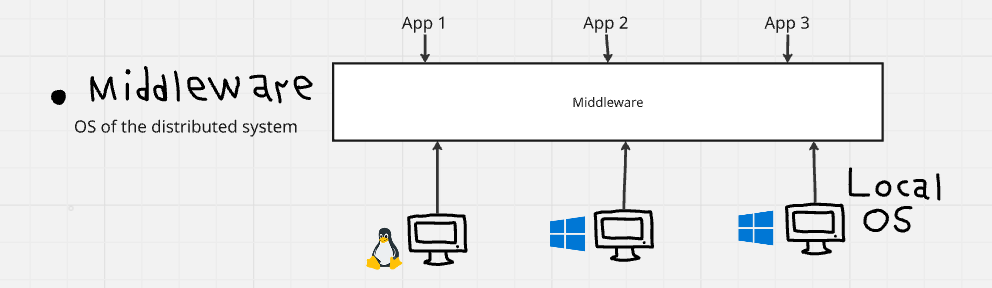
\includegraphics[width=0.5\textwidth]{images/middleware.png} \\

\section{Distribution Systems for Pervasive computing}

\subsection{Ubiquitous Computing System}

Pervasive and common

\subsection{Mobile Computing System}

Pervasive but emphasis is on fact that devices are inherently mobile.

\subsection{Sensor networks}

Persasive and emphasis on the actual collaborating and sensing of the environment.

\end{document}